\chapter{هندسه}

\index{geometry@هندسه}

در مسائل هندسی، یافتن روشی برای حل که پیاده‌سازی راحتی داشته باشد و حالت‌های خاص آن کم باشد، اغلب چالش‌برانگیز است.

به عنوان مثال، مسئله‌ای را در نظر بگیرید که در آن رأس‌های یک چهارضلعی (چندضلعی با چهار رأس) داده شده است و وظیفه ما محاسبه مساحت آن است. به عنوان نمونه، یک ورودی ممکن برای مسئله به صورت زیر است:

\begin{center}
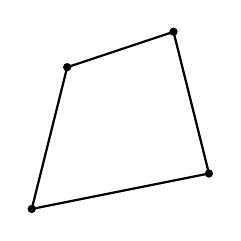
\begin{tikzpicture}[scale=0.45]

\draw[fill] (6,2) circle [radius=0.1];
\draw[fill] (5,6) circle [radius=0.1];
\draw[fill] (2,5) circle [radius=0.1];
\draw[fill] (1,1) circle [radius=0.1];
\draw[thick] (6,2) -- (5,6) -- (2,5) -- (1,1) -- (6,2);
\end{tikzpicture}
\end{center}
یک روش برای حل مسئله، تقسیم چهارضلعی به دو مثلث به وسیله یک خط مستقیم بین دو رأس روبه‌رو است:
\begin{center}
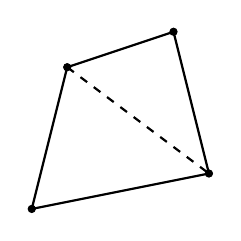
\begin{tikzpicture}[scale=0.45]

\draw[fill] (6,2) circle [radius=0.1];
\draw[fill] (5,6) circle [radius=0.1];
\draw[fill] (2,5) circle [radius=0.1];
\draw[fill] (1,1) circle [radius=0.1];

\draw[thick] (6,2) -- (5,6) -- (2,5) -- (1,1) -- (6,2);
\draw[dashed,thick] (2,5) -- (6,2);
\end{tikzpicture}
\end{center}
پس از این، جمع زدن مساحت مثلث‌ها کافی است. مساحت یک مثلث را می‌توان مثلاً با استفاده از \key{فرمول هرون} محاسبه کرد:
%\footnote{Heron of Alexandria (c. 10--70) was a Greek mathematician.}
\[ \sqrt{s (s-a) (s-b) (s-c)},\]
که در آن $a$، $b$ و $c$ طول اضلاع مثلث هستند و $s=(a+b+c)/2$.
\index{Heron's formula@فرمول هرون}

این یک روش ممکن برای حل مسئله است، اما یک دام وجود دارد: چگونه چهارضلعی را به مثلث‌ها تقسیم کنیم؟ مشخص می‌شود گاهی نمی‌توانیم صرفاً دو رأس روبه‌روی دلخواه را انتخاب کنیم. به عنوان مثال، در وضعیت زیر، خط تقسیم \emph{خارج} چهارضلعی قرار می‌گیرد:
\begin{center}
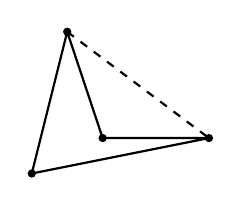
\begin{tikzpicture}[scale=0.45]

\draw[fill] (6,2) circle [radius=0.1];
\draw[fill] (3,2) circle [radius=0.1];
\draw[fill] (2,5) circle [radius=0.1];
\draw[fill] (1,1) circle [radius=0.1];
\draw[thick] (6,2) -- (3,2) -- (2,5) -- (1,1) -- (6,2);

\draw[dashed,thick] (2,5) -- (6,2);
\end{tikzpicture}
\end{center}
با این حال، روش دیگر برای رسم خط کار می‌کند:
\begin{center}
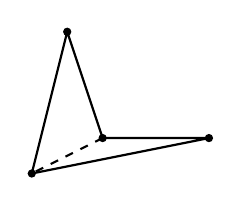
\begin{tikzpicture}[scale=0.45]

\draw[fill] (6,2) circle [radius=0.1];
\draw[fill] (3,2) circle [radius=0.1];
\draw[fill] (2,5) circle [radius=0.1];
\draw[fill] (1,1) circle [radius=0.1];
\draw[thick] (6,2) -- (3,2) -- (2,5) -- (1,1) -- (6,2);

\draw[dashed,thick] (3,2) -- (1,1);
\end{tikzpicture}
\end{center}
برای انسان انتخاب خط درست بدیهی است، اما کامپیوتر با موقعیت سختی روبه‌رو می‌شود.

با این حال، می‌توان مسأله را با روشی دیگر حل کرد که کار برنامه‌نویس را راحت‌تر می‌کند.
به‌طور مشخص، رابطه کلی
\[x_1y_2-x_2y_1+x_2y_3-x_3y_2+x_3y_4-x_4y_3+x_4y_1-x_1y_4\]
مساحت چهارضلعی با رأس‌های
$(x_1,y_1)$،
$(x_2,y_2)$،
$(x_3,y_3)$ و
$(x_4,y_4)$
را محاسبه می‌کند.
پیاده‌سازی این فرمول آسان است، حالت خاص ندارد و حتی قابل تعمیم به \emph{تمام} چندضلعی‌ها است.

\section{اعداد مختلط}

\index{complex number}
\index{point}
\index{vector}

یک \key{عدد مختلط} عددی به فرم $x+y i$ است
که در آن $i = \sqrt{-1}$ \key{واحد موهومی} است.
تعبیر هندسی عدد مختلط،
نمایش نقطه دوبعدی $(x,y)$
یا برداری از مبدأ به نقطه $(x,y)$ است.

برای نمونه، $4+2i$ با نقطه و بردار زیر تطابق دارد:

\begin{center}
\begin{tikzpicture}[scale=0.45]

\draw[->,thick] (-5,0)--(5,0);
\draw[->,thick] (0,-5)--(0,5);

\draw[fill] (4,2) circle [radius=0.1];
\draw[->,thick] (0,0)--(4-0.1,2-0.1);

\node at (4,2.8) {$(4,2)$};
\end{tikzpicture}
\end{center}

\index{complex@\texttt{complex}}

کلاس اعداد مختلط در سی‌پلاس‌پلاس (\texttt{complex}) در حل مسائل هندسی کاربرد دارد.
با این کلاس می‌توان نقطه‌ها و بردارها را به شکل اعداد مختلط ذخیره کرد؛
همچنین ابزارهای هندسی مفیدی دارد.

در کد زیر، \texttt{C} نوع داده مختصات و \texttt{P} نوع داده نقطه یا بردار است.
به علاوه، ماکروهای \texttt{X} و \texttt{Y} برای ارجاع به مختصات x و y تعریف شده‌اند.

\begin{lstlisting}
typedef long long C;
typedef complex<C> P;
#define X real()
#define Y imag()
\end{lstlisting}

برای مثال، کد زیر نقطه $p=(4,2)$ را تعریف می‌کند و مختصات x و y آن را چاپ می‌کند:

\begin{lstlisting}
P p = {4,2};
cout << p.X << " " << p.Y << "\n"; // 4 2
\end{lstlisting}

کد زیر بردارهای $v=(3,1)$ و $u=(2,2)$ را تعریف می‌کند و سپس مجموع $s=v+u$ را به دست می‌آورد:

\begin{lstlisting}
P v = {3,1};
P u = {2,2};
P s = v+u;
cout << s.X << " " << s.Y << "\n"; // 5 3
\end{lstlisting}

در عمل،
نوع مناسب برای مختصات معمولاً
\texttt{long long} (عدد صحیح) یا \texttt{long double}
(عدد حقیقی) است.
بهتر است تا حد امکان از اعداد صحیح استفاده شود
زیرا محاسبات آن‌ها دقیق است.
در صورت نیاز به اعداد حقیقی،
خطای دقت را هنگام مقایسه‌ها باید در نظر گرفت.
روش امن برای بررسی برابری دو عدد حقیقی $a$ و $b$،
مقایسه به صورت $|a-b|<\epsilon$ است
که در آن $\epsilon$ مقداری بسیار کوچک است (مثلاً $\epsilon=10^{-9}$).

\subsubsection*{توابع}

در مثال‌های زیر، نوع داده مختصات
\texttt{long double} است.

تابع $\texttt{abs}(v)$ طول $|v|$ بردار $v=(x,y)$ را با فرمول $\sqrt{x^2+y^2}$ محاسبه می‌کند.
همچنین برای محاسبه فاصله بین نقاط $(x_1,y_1)$ و $(x_2,y_2)$ کاربرد دارد؛
فاصله برابر طول بردار $(x_2-x_1,y_2-y_1)$ است.

کد زیر فاصله بین نقاط $(4,2)$ و $(3,-1)$ را محاسبه می‌کند:
\begin{lstlisting}
P a = {4,2};
P b = {3,-1};
cout << abs(b-a) << "\n"; // 3.16228
\end{lstlisting}

تابع $\texttt{arg}(v)$ زاویه بردار $v=(x,y)$ نسبت به محور x را می‌دهد.
زاویه بر حسب رادیان است؛
هر $r$ رادیان برابر $180 r/\pi$ درجه است.
زاویه بردار رو به راست 0 است؛
جهت عقربه‌های ساعت کاهش و پادساعت‌گرد افزایش می‌یابد.

تابع $\texttt{polar}(s,a)$ برداری با طول $s$ و زاویه $a$ می‌سازد.
دوران بردار به اندازه زاویه $a$ با ضرب آن در برداری با طول 1 و زاویه $a$ انجام می‌شود.

کد زیر زاویه بردار $(4,2)$ را می‌گیرد، آن را $1/2$ رادیان پادساعت‌گرد می‌چرخاند و زاویه جدید را چاپ می‌کند:

\begin{lstlisting}
P v = {4,2};
cout << arg(v) << "\n"; // 0.463648
v *= polar(1.0,0.5);
cout << arg(v) << "\n"; // 0.963648
\end{lstlisting}

\section{نقاط و خطوط}

\index{cross product}

\key{ضرب خارجی} (cross product) $a \times b$ دو بردار $a=(x_1,y_1)$ و $b=(x_2,y_2)$ با فرمول $x_1 y_2 - x_2 y_1$ محاسبه می‌شود.
ضرب خارجی مشخص می‌کند بردار $b$ پس از بردار $a$،
به چپ می‌پیچد (مقدار مثبت)، مستقیم می‌رود (صفر)،
یا به راست می‌پیچد (مقدار منفی).

تصویر زیر این حالت‌ها را نشان می‌دهد:
\begin{center}
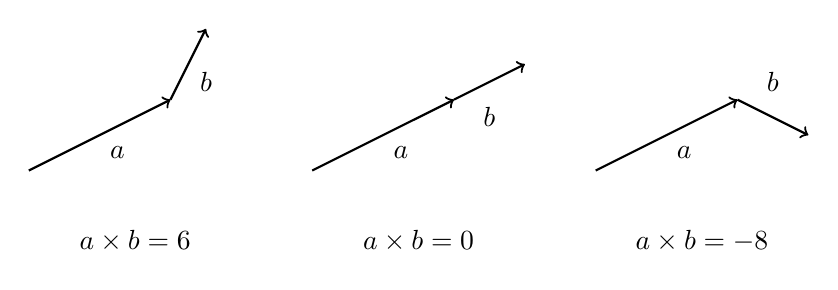
\begin{tikzpicture}[scale=0.45]

\draw[->,thick] (0,0)--(4,2);
\draw[->,thick] (4,2)--(4+1,2+2);

\node at (2.5,0.5) {$a$};
\node at (5,2.5) {$b$};

\node at (3,-2) {$a \times b = 6$};

\draw[->,thick] (8+0,0)--(8+4,2);
\draw[->,thick] (8+4,2)--(8+4+2,2+1);

\node at (8+2.5,0.5) {$a$};
\node at (8+5,1.5) {$b$};

\node at (8+3,-2) {$a \times b = 0$};

\draw[->,thick] (16+0,0)--(16+4,2);
\draw[->,thick] (16+4,2)--(16+4+2,2-1);

\node at (16+2.5,0.5) {$a$};
\node at (16+5,2.5) {$b$};

\node at (16+3,-2) {$a \times b = -8$};
\end{tikzpicture}
\end{center}

\noindent
مثال: در حالت اول $a=(4,2)$ و $b=(1,2)$ است.
کد زیر ضرب خارجی را با کلاس \texttt{complex} حساب می‌کند:

\begin{lstlisting}
P a = {4,2};
P b = {1,2};
C p = (conj(a)*b).Y; // 6
\end{lstlisting}

کد کار می‌کند چون تابع \texttt{conj} مولفه y بردار را قرینه می‌کند؛
از ضرب دو بردار $(x_1,-y_1)$ و $(x_2,y_2)$، مولفه y حاصل برابر $x_1 y_2 - x_2 y_1$ می‌شود.

\subsubsection{موقعیت نقطه}

ضرب خارجی برای تعیین قرارگیری نقطه در سمت چپ یا راست خط کاربرد دارد.
خط از نقاط $s_1$ و $s_2$ می‌گذرد؛ دید از $s_1$ به سمت $s_2$ است و نقطه $p$ بررسی می‌شود.

برای مثال، در تصویر زیر،
$p$ در سمت چپ خط قرار دارد:
\begin{center}
\begin{tikzpicture}[scale=0.45]
\draw[dashed,thick,->] (0,-3)--(12,6);
\draw[fill] (4,0) circle [radius=0.1];
\draw[fill] (8,3) circle [radius=0.1];
\draw[fill] (5,3) circle [radius=0.1];
\node at (4,-1) {$s_1$};
\node at (8,2) {$s_2$};
\node at (5,4) {$p$};
\end{tikzpicture}
\end{center}

ضرب خارجی $(p-s_1) \times (p-s_2)$
موقعیت نقطه $p$ را مشخص می‌کند.
اگر ضرب خارجی مثبت باشد،
$p$ در سمت چپ قرار دارد،
و اگر ضرب خارجی منفی باشد،
$p$ در سمت راست قرار دارد.
در نهایت، اگر ضرب خارجی صفر باشد،
نقاط $s_1$، $s_2$ و $p$ روی یک خط قرار دارند.

\subsubsection{تقاطع پاره‌خط‌ها}

\index{تقاطع پاره‌خط‌ها}

در ادامه مسئله بررسی اینکه آیا دو پاره‌خط
$ab$ و $cd$ متقاطع هستند یا خیر را بررسی می‌کنیم. حالت‌های ممکن عبارتند از:

\textit{حالت ۱:}
پاره‌خط‌ها روی یک خط قرار دارند
و با یکدیگر همپوشانی دارند.
در این حالت، بی‌نهایت نقطه تقاطع وجود دارد.
برای مثال، در تصویر زیر،
تمام نقاط بین $c$ و $b$ نقاط تقاطع هستند:
\begin{center}
\begin{tikzpicture}[scale=0.9]
\draw (1.5,1.5)--(6,3);
\draw (0,1)--(4.5,2.5);
\draw[fill] (0,1) circle [radius=0.05];
\node at (0,0.5) {$a$};
\draw[fill] (1.5,1.5) circle [radius=0.05];
\node at (6,2.5) {$d$};
\draw[fill] (4.5,2.5) circle [radius=0.05];
\node at (1.5,1) {$c$};
\draw[fill] (6,3) circle [radius=0.05];
\node at (4.5,2) {$b$};
\end{tikzpicture}
\end{center}

در این حالت، می‌توان از ضرب خارجی برای بررسی اینکه آیا همه نقاط روی یک خط هستند استفاده کرد.
سپس، می‌توان نقاط را مرتب کرد و بررسی نمود که آیا پاره‌خط‌ها همپوشانی دارند یا خیر.

\textit{حالت ۲:}
پاره‌خط‌ها رأس مشترکی دارند
که تنها نقطه تقاطع است.
برای مثال، در تصویر زیر نقطه تقاطع $b=c$ است:

\begin{center}
\begin{tikzpicture}[scale=0.9]
\draw (0,0)--(4,2);
\draw (4,2)--(6,1);
\draw[fill] (0,0) circle [radius=0.05];
\draw[fill] (4,2) circle [radius=0.05];
\draw[fill] (6,1) circle [radius=0.05];

\node at (0,0.5) {$a$};
\node at (4,2.5) {$b=c$};
\node at (6,1.5) {$d$};
\end{tikzpicture}
\end{center}

بررسی این حالت ساده است، زیرا
تنها چهار احتمال برای نقطه تقاطع وجود دارد:
$a=c$، $a=d$، $b=c$ و $b=d$.

\textit{حالت ۳:}
دقیقاً یک نقطه تقاطع وجود دارد
که رأس هیچ‌یک از پاره‌خط‌ها نیست.
در تصویر زیر، نقطه $p$ نقطه تقاطع است:
\begin{center}
\begin{tikzpicture}[scale=0.9]
\draw (0,1)--(6,3);
\draw (2,4)--(4,0);
\draw[fill] (0,1) circle [radius=0.05];
\node at (0,0.5) {$c$};
\draw[fill] (6,3) circle [radius=0.05];
\node at (6,2.5) {$d$};
\draw[fill] (2,4) circle [radius=0.05];
\node at (1.5,3.5) {$a$};
\draw[fill] (4,0) circle [radius=0.05];
\node at (4,-0.4) {$b$};
\draw[fill] (3,2) circle [radius=0.05];
\node at (3,1.5) {$p$};
\end{tikzpicture}
\end{center}

در این حالت، پاره‌خط‌ها دقیقاً زمانی یکدیگر را قطع می‌کنند
که هر دو نقطه $c$ و $d$ در دو سمت مختلف خط گذرنده از $a$ و $b$ باشند،
و نقاط $a$ و $b$ در دو سمت مختلف خط گذرنده از $c$ و $d$ قرار گیرند.
می‌توان از ضرب خارجی برای بررسی این موضوع استفاده کرد.

\subsubsection{فاصله نقطه از خط}

یکی دیگر از کاربردهای ضرب خارجی این است که
مساحت مثلث را می‌توان با استفاده از فرمول
\[\frac{| (a-c) \times (b-c) |}{2},\]
محاسبه کرد، که در آن $a$، $b$ و $c$ رأس‌های مثلث هستند.
با استفاده از این نکته، می‌توان فرمولی برای محاسبه کوتاه‌ترین فاصله بین یک نقطه و یک خط به دست آورد.
برای نمونه، در تصویر زیر $d$ کوتاه‌ترین فاصله بین نقطه $p$ و خط تعریف‌شده توسط نقاط $s_1$ و $s_2$ است:
\begin{center}
\begin{tikzpicture}[scale=0.75]
\draw (-2,-1)--(6,3);
\draw[dashed] (1,4)--(2.40,1.2);
\node at (0,-0.5) {$s_1$};
\node at (4,1.5) {$s_2$};
\node at (0.5,4) {$p$};
\node at (2,2.7) {$d$};
\draw[fill] (0,0) circle [radius=0.05];
\draw[fill] (4,2) circle [radius=0.05];
\draw[fill] (1,4) circle [radius=0.05];
\end{tikzpicture}
\end{center}

مساحت مثلثی که رأس‌های آن
$s_1$، $s_2$ و $p$ هستند را می‌توان به دو روش محاسبه کرد:
این مساحت هم برابر $\frac{1}{2} |s_2-s_1| d$ است
و هم برابر $\frac{1}{2} ((s_1-p) \times (s_2-p))$.
بنابراین، کوتاه‌ترین فاصله عبارت است از:
\[ d = \frac{(s_1-p) \times (s_2-p)}{|s_2-s_1|} .\]

\subsubsection{نقطه درون چندضلعی}

اکنون مسئله بررسی قرار داشتن یک نقطه درون یا بیرون چندضلعی را در نظر بگیرید.
برای نمونه، در تصویر زیر نقطه $a$ درون چندضلعی و نقطه $b$ بیرون چندضلعی قرار دارد.

\begin{center}
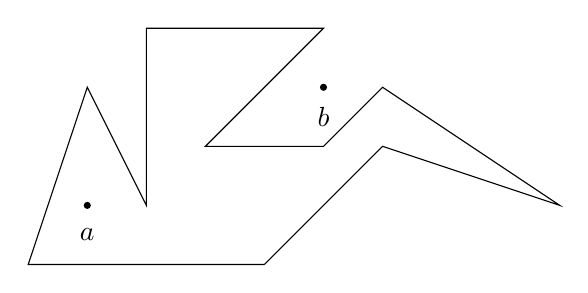
\begin{tikzpicture}[scale=0.75]
%\draw (0,0)--(2,-2)--(3,1)--(5,1)--(2,3)--(1,2)--(-1,2)--(1,4)--(-2,4)--(-2,1)--(-3,3)--(-4,0)--(0,0);
\draw (0,0)--(2,2)--(5,1)--(2,3)--(1,2)--(-1,2)--(1,4)--(-2,4)--(-2,1)--(-3,3)--(-4,0)--(0,0);

\draw[fill] (-3,1) circle [radius=0.05];
\node at (-3,0.5) {$a$};
\draw[fill] (1,3) circle [radius=0.05];
\node at (1,2.5) {$b$};
\end{tikzpicture}
\end{center}

یک روش مناسب برای حل مسئله،
تاباندن یک \emph{پرتو} از نقطه در جهتی دلخواه
و شمارش تعداد دفعات برخورد آن با مرز چندضلعی است.
اگر این تعداد فرد باشد،
نقطه درون چندضلعی قرار دارد،
و اگر زوج باشد،
نقطه بیرون چندضلعی است.

\begin{samepage}
برای نمونه، می‌توان پرتوهای زیر را تاباند:
\begin{center}
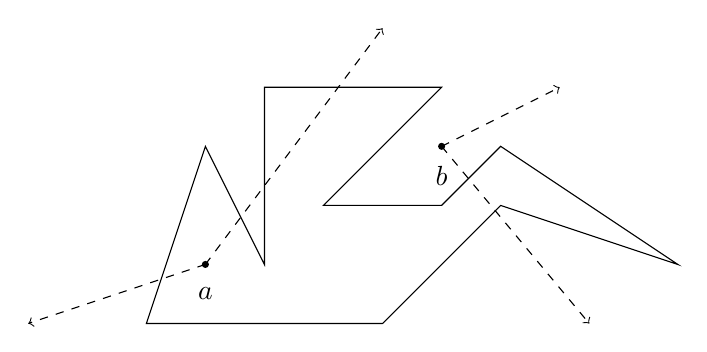
\begin{tikzpicture}[scale=0.75]
\draw (0,0)--(2,2)--(5,1)--(2,3)--(1,2)--(-1,2)--(1,4)--(-2,4)--(-2,1)--(-3,3)--(-4,0)--(0,0);

\draw[fill] (-3,1) circle [radius=0.05];
\node at (-3,0.5) {$a$};
\draw[fill] (1,3) circle [radius=0.05];
\node at (1,2.5) {$b$};

\draw[dashed,->] (-3,1)--(-6,0);
\draw[dashed,->] (-3,1)--(0,5);

\draw[dashed,->] (1,3)--(3.5,0);
\draw[dashed,->] (1,3)--(3,4);
\end{tikzpicture}
\end{center}
\end{samepage}

پرتوهای خارج‌شده از $a$ مرز چندضلعی را ۱ و ۳ بار قطع می‌کنند،
بنابراین $a$ درون چندضلعی قرار دارد.
به‌همین ترتیب، پرتوهای خارج‌شده از $b$ مرز چندضلعی را ۰ و ۲ بار قطع می‌کنند،
بنابراین $b$ بیرون چندضلعی است.

\section{مساحت چندضلعی}

فرمول کلی برای محاسبه مساحت یک چندضلعی،
که گاهی \key{فرمول بند کفش} نامیده می‌شود،
به این صورت است: \index{فرمول بند کفش}
\[\frac{1}{2} |\sum_{i=1}^{n-1} (p_i \times p_{i+1})| =
\frac{1}{2} |\sum_{i=1}^{n-1} (x_i y_{i+1} - x_{i+1} y_i)|, \]
در اینجا رأس‌ها به ترتیب
$p_1=(x_1,y_1)$، $p_2=(x_2,y_2)$، $\ldots$، $p_n=(x_n,y_n)$ هستند
به‌گونه‌ای که $p_i$ و $p_{i+1}$ رأس‌های مجاور روی مرز چندضلعی باشند،
و رأس اول و آخر یکسان است، یعنی $p_1=p_n$.

برای مثال، مساحت چندضلعی
\begin{center}
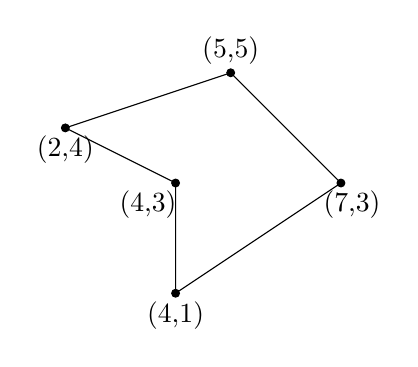
\begin{tikzpicture}[scale=0.7]
\filldraw (4,1.4) circle (2pt);
\filldraw (7,3.4) circle (2pt);
\filldraw (5,5.4) circle (2pt);
\filldraw (2,4.4) circle (2pt);
\filldraw (4,3.4) circle (2pt);
\node (1) at (4,1) {(4,1)};
\node (2) at (7.2,3) {(7,3)};
\node (3) at (5,5.8) {(5,5)};
\node (4) at (2,4) {(2,4)};
\node (5) at (3.5,3) {(4,3)};
\path[draw] (4,1.4) -- (7,3.4) -- (5,5.4) -- (2,4.4) -- (4,3.4) -- (4,1.4);
\end{tikzpicture}
\end{center}
برابر است با:
\[\frac{|(2\cdot5-5\cdot4)+(5\cdot3-7\cdot5)+(7\cdot1-4\cdot3)+(4\cdot3-4\cdot1)+(4\cdot4-2\cdot3)|}{2} = 17/2.\]

ایده این فرمول بررسی ذوزنقه‌هایی است
که یک ضلع آن‌ها ضلعی از چندضلعی است،
و ضلع دیگر روی خط افقی $y=0$ قرار دارد.
برای مثال:
\begin{center}
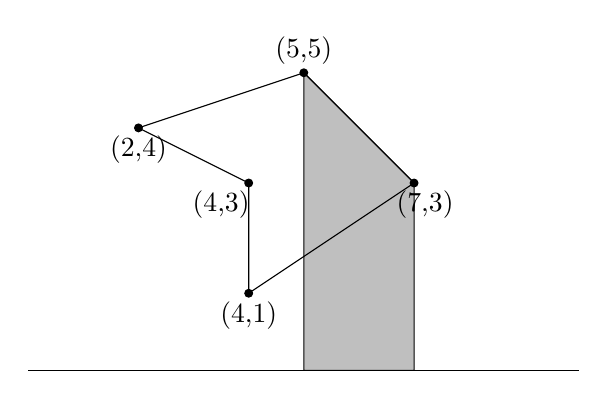
\begin{tikzpicture}[scale=0.7]
\path[draw,fill=lightgray] (5,5.4) -- (7,3.4) -- (7,0) -- (5,0) -- (5,5.4);
\filldraw (4,1.4) circle (2pt);
\filldraw (7,3.4) circle (2pt);
\filldraw (5,5.4) circle (2pt);
\filldraw (2,4.4) circle (2pt);
\filldraw (4,3.4) circle (2pt);
\node (1) at (4,1) {(4,1)};
\node (2) at (7.2,3) {(7,3)};
\node (3) at (5,5.8) {(5,5)};
\node (4) at (2,4) {(2,4)};
\node (5) at (3.5,3) {(4,3)};
\path[draw] (4,1.4) -- (7,3.4) -- (5,5.4) -- (2,4.4) -- (4,3.4) -- (4,1.4);
\draw (0,0) -- (10,0);
\end{tikzpicture}
\end{center}
مساحت چنین ذوزنقه‌ای برابر است با
\[(x_{i+1}-x_{i}) \frac{y_i+y_{i+1}}{2},\]
که در آن رأس‌های چندضلعی $p_i$ و $p_{i+1}$ هستند.
اگر $x_{i+1}>x_{i}$ باشد، مساحت مثبت است،
و اگر $x_{i+1}<x_{i}$ باشد، مساحت منفی است.

مساحت چندضلعی برابر با مجموع مساحت‌های
همه این ذوزنقه‌ها است که فرمول زیر را به‌دست می‌دهد:
\[|\sum_{i=1}^{n-1} (x_{i+1}-x_{i}) \frac{y_i+y_{i+1}}{2}| =
\frac{1}{2} |\sum_{i=1}^{n-1} (x_i y_{i+1} - x_{i+1} y_i)|.\]

توجه کنید که قدر مطلق مجموع گرفته می‌شود،
زیرا بسته به اینکه در جهت عقربه‌های ساعت یا پادساعت‌گرد
روی مرز چندضلعی حرکت کنیم، مقدار مجموع ممکن است مثبت یا منفی باشد.

\subsubsection{قضیه پیک}

\index{قضیه پیک}

\key{قضیه پیک} روش دیگر محاسبه مساحت چندضلعی ارائه دهد، به شرطی که همه رأس‌های چندضلعی مختصات صحیح داشته باشند.
طبق قضیه پیک، مساحت چندضلعی برابر است با:
\[ a + b/2 -1,\]
که در آن $a$ تعداد نقاط صحیح درون چندضلعی و $b$ تعداد نقاط صحیح روی مرز چندضلعی است.

برای مثال، مساحت چندضلعی
\begin{center}
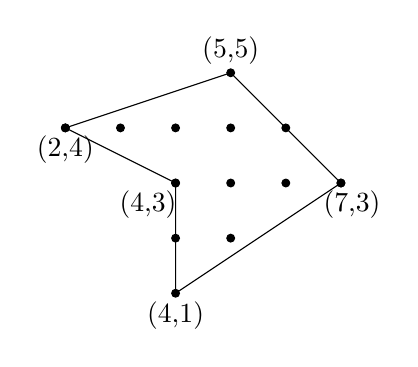
\begin{tikzpicture}[scale=0.7]
\filldraw (4,1.4) circle (2pt);
\filldraw (7,3.4) circle (2pt);
\filldraw (5,5.4) circle (2pt);
\filldraw (2,4.4) circle (2pt);
\filldraw (4,3.4) circle (2pt);
\node (1) at (4,1) {(4,1)};
\node (2) at (7.2,3) {(7,3)};
\node (3) at (5,5.8) {(5,5)};
\node (4) at (2,4) {(2,4)};
\node (5) at (3.5,3) {(4,3)};
\path[draw] (4,1.4) -- (7,3.4) -- (5,5.4) -- (2,4.4) -- (4,3.4) -- (4,1.4);

\filldraw (2,4.4) circle (2pt);
\filldraw (3,4.4) circle (2pt);
\filldraw (4,4.4) circle (2pt);
\filldraw (5,4.4) circle (2pt);
\filldraw (6,4.4) circle (2pt);

\filldraw (4,3.4) circle (2pt);
\filldraw (5,3.4) circle (2pt);
\filldraw (6,3.4) circle (2pt);
\filldraw (7,3.4) circle (2pt);

\filldraw (4,2.4) circle (2pt);
\filldraw (5,2.4) circle (2pt);
\end{tikzpicture}
\end{center}
برابر است با $6+7/2-1=17/2$.

\section{تابع‌های فاصله}

\index{تابع فاصله}
\index{فاصله اقلیدسی}
\index{فاصله منهتن}

یک \key{تابع فاصله} فاصله بین دو نقطه را مشخص کند.
تابع فاصله معمول \key{فاصله اقلیدسی} است که فاصله بین نقاط $(x_1,y_1)$ و $(x_2,y_2)$ در آن برابر است با:
\[\sqrt{(x_2-x_1)^2+(y_2-y_1)^2}.\]
تابع فاصله جایگزین دیگر \key{فاصله منهتن} است
که فاصله بین نقاط $(x_1,y_1)$ و $(x_2,y_2)$ در آن برابر است با:
\[|x_1-x_2|+|y_1-y_2|.\]
\begin{samepage}
برای مثال، تصویر زیر را ببینید:
\begin{center}
\begin{tikzpicture}

\draw[fill] (2,1) circle [radius=0.05];
\draw[fill] (5,2) circle [radius=0.05];

\node at (2,0.5) {$(2,1)$};
\node at (5,1.5) {$(5,2)$};

\draw[dashed] (2,1) -- (5,2);

\draw[fill] (5+2,1) circle [radius=0.05];
\draw[fill] (5+5,2) circle [radius=0.05];

\node at (5+2,0.5) {$(2,1)$};
\node at (5+5,1.5) {$(5,2)$};

\draw[dashed] (5+2,1) -- (5+2,2);
\draw[dashed] (5+2,2) -- (5+5,2);

\node at (3.5,-0.5) {فاصله اقلیدسی};
\node at (5+3.5,-0.5) {فاصله منهتن};
\end{tikzpicture}
\end{center}
\end{samepage}
فاصله اقلیدسی بین نقاط برابر است با:
\[\sqrt{(5-2)^2+(2-1)^2}=\sqrt{10}\]
و فاصله منهتن برابر است با:
\[|5-2|+|2-1|=4.\]
تصویر زیر ناحیه‌هایی با فاصله حداکثر ۱ از نقطه مرکز را با استفاده از فواصل اقلیدسی و منهتن نشان دهد:
\begin{center}
\begin{tikzpicture}

\draw[fill=gray!20] (0,0) circle [radius=1];
\draw[fill] (0,0) circle [radius=0.05];

\node at (0,-1.5) {فاصله اقلیدسی};

\draw[fill=gray!20] (5+0,1) -- (5-1,0) -- (5+0,-1) -- (5+1,0) -- (5+0,1);
\draw[fill] (5,0) circle [radius=0.05];
\node at (5,-1.5) {فاصله منهتن};
\end{tikzpicture}
\end{center}

\subsubsection{دوران دستگاه مختصات}

حل برخی مسئله‌ها با فاصله منهتن ساده‌تر از فاصله اقلیدسی است.
مثال: $n$ نقطه در صفحه دو‌بعدی داده شده است.
هدف: محاسبه بیشینه فاصله منهتن بین هر دو نقطه.

مجموعه نقاط زیر را در نظر بگیرید:
\begin{center}
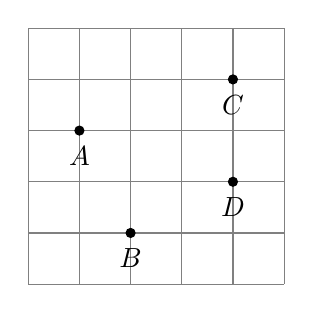
\begin{tikzpicture}[scale=0.65]
\draw[color=gray] (-1,-1) grid (4,4);

\filldraw (0,2) circle (2.5pt);
\filldraw (3,3) circle (2.5pt);
\filldraw (1,0) circle (2.5pt);
\filldraw (3,1) circle (2.5pt);

\node at (0,1.5) {$A$};
\node at (3,2.5) {$C$};
\node at (1,-0.5) {$B$};
\node at (3,0.5) {$D$};
\end{tikzpicture}
\end{center}
بیشینه فاصله منهتن برابر ۵ بین نقاط $B$ و $C$ است:
\begin{center}
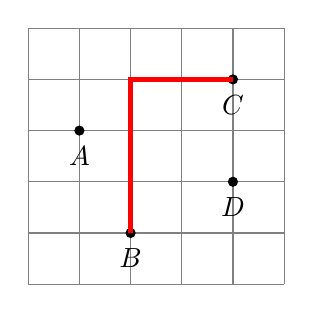
\begin{tikzpicture}[scale=0.65]
\draw[color=gray] (-1,-1) grid (4,4);

\filldraw (0,2) circle (2.5pt);
\filldraw (3,3) circle (2.5pt);
\filldraw (1,0) circle (2.5pt);
\filldraw (3,1) circle (2.5pt);

\node at (0,1.5) {$A$};
\node at (3,2.5) {$C$};
\node at (1,-0.5) {$B$};
\node at (3,0.5) {$D$};

\path[draw=red,thick,line width=2pt] (1,0) -- (1,3) -- (3,3);
\end{tikzpicture}
\end{center}

تکنیک کاربردی: چرخش ۴۵ درجه‌ای مختصات.
نقطه $(x,y)$ تبدیل می‌شود به $(x+y,y-x)$.
پس از چرخش نقاط بالا:

\begin{center}
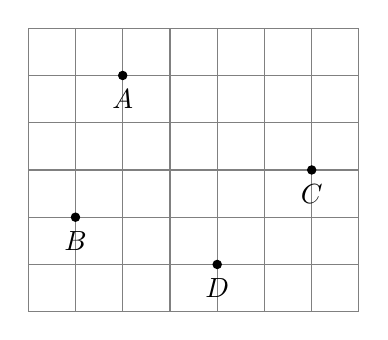
\begin{tikzpicture}[scale=0.6]
\draw[color=gray] (0,-3) grid (7,3);

\filldraw (2,2) circle (2.5pt);
\filldraw (6,0) circle (2.5pt);
\filldraw (1,-1) circle (2.5pt);
\filldraw (4,-2) circle (2.5pt);

\node at (2,1.5) {$A$};
\node at (6,-0.5) {$C$};
\node at (1,-1.5) {$B$};
\node at (4,-2.5) {$D$};
\end{tikzpicture}
\end{center}
بیشینه فاصله این‌گونه می‌شود:
\begin{center}
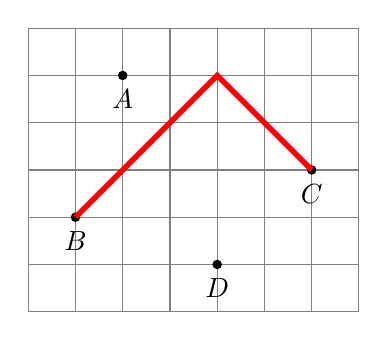
\begin{tikzpicture}[scale=0.6]
\draw[color=gray] (0,-3) grid (7,3);

\filldraw (2,2) circle (2.5pt);
\filldraw (6,0) circle (2.5pt);
\filldraw (1,-1) circle (2.5pt);
\filldraw (4,-2) circle (2.5pt);

\node at (2,1.5) {$A$};
\node at (6,-0.5) {$C$};
\node at (1,-1.5) {$B$};
\node at (4,-2.5) {$D$};

\path[draw=red,thick,line width=2pt] (1,-1) -- (4,2) -- (6,0);
\end{tikzpicture}
\end{center}

نقاط $p_1=(x_1,y_1)$ و $p_2=(x_2,y_2)$ دارای مختصات چرخانده‌شده $p'_1=(x'_1,y'_1)$ و $p'_2=(x'_2,y'_2)$ هستند.
دو روش بیان فاصله منهتن بین $p_1$ و $p_2$:
\[|x_1-x_2|+|y_1-y_2| = \max(|x'_1-x'_2|,|y'_1-y'_2|)\]

مثال: اگر $p_1=(1,0)$ و $p_2=(3,3)$،
مختصات چرخانده‌شده $p'_1=(1,-1)$ و $p'_2=(6,0)$ است
و فاصله منهتن برابر است با:
\[|1-3|+|0-3| = \max(|1-6|,|-1-0|) = 5.\]

مختصات چرخانده‌شده کار با فاصله منهتن را ساده می‌کند؛ مولفه‌های x و y جداگانه بررسی می‌شوند.
برای بیشینه‌سازی فاصله منهتن دو نقطه، دو نقطه‌ای را بیابید که مقدار زیر را بیشینه کنند:
\[\max(|x'_1-x'_2|,|y'_1-y'_2|).\]
محاسبه ساده است؛ تفاضل افقی یا عمودی در مختصات جدید باید بیشینه باشد.